     
\documentclass[addpoints]{exam}
    


\usepackage{amsfonts}
\usepackage{tikz}
\usepackage{amsmath}

\usetikzlibrary{arrows,shapes}

\sloppy


\begin{document}

  \pagestyle{headandfoot}
  \runningheadrule
  \firstpageheader{ Math 184A }{ Homework 5 }{ May 26, 2019 }
  \runningheader{ Math 184A }{ Homework 5, Page \thepage\ of \numpages}{ May 26, 2019 }

  \firstpagefooter{}{}{}
  \runningfooter{}{}{}
  \begin{flushright}
    \makebox[0.4\textwidth]{Name: \enspace\hrulefill}

    \vspace{0.2in}
    \makebox[0.4\textwidth]{Pid:\enspace\hrulefill}
  \end{flushright}

  \begin{questions}
    \question[10]
      Let $G$ be a graph such that degrees of all the vertices are equal to $4$.
			Show that one may color all the edges into black and white so that every
			vertex is incident to two vertices of each color.

      \begin{solution}[\stretch{1}]
      \end{solution}
      \newpage
    \question[10]
      Show that the following graph has no Hamiltonian cycle.
			
			\begin{figure}[h]
				\centering
				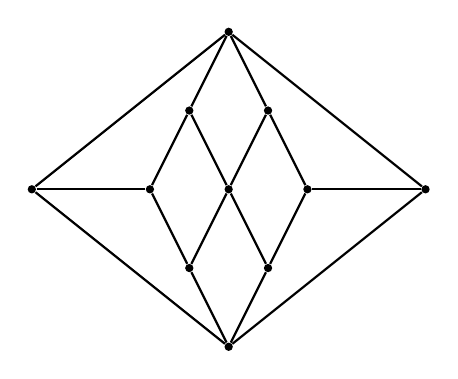
\begin{tikzpicture}[scale=0.5, auto,swap]
					% Draw a 7,11 network
					% First we draw the vertices
					\foreach \pos/\name in {{(0,0)/1}, {(3,0)/2}, {(5,0)/3},
			        	                    {(7,0)/4}, {(10,0)/5}, {(4,2)/6}, {(6,2)/7},
							    {(5,4)/8}, {(4,-2)/9}, {(6,-2)/10}, {(5,-4)/11}}
						\node[circle,fill=black,minimum size=3pt,inner sep=0pt] (\name) at \pos {};
					\foreach \source/ \dest in {1/2, 4/5, 2/6, 2/9, 3/6, 3/9, 3/7,
							    3/10, 4/7, 4/10, 8/6, 8/7, 11/9, 11/10, 1/8, 1/11, 5/8, 5/11}
						\path[draw,thick,-] (\source) -- (\dest);
				\end{tikzpicture}
			\end{figure}

      \begin{solution}[\stretch{1}]
      \end{solution}
      \newpage
  \end{questions}
\end{document}